\documentclass[hidelinks,a4paper,12pt]{article}
\addtolength{\oddsidemargin}{-1.cm}
\addtolength{\textwidth}{2cm}
\addtolength{\topmargin}{-2cm}
\addtolength{\textheight}{3.5cm}
\newcommand{\HRule}{\rule{\linewidth}{0.5mm}}
\makeindex

\usepackage{longtable}
\usepackage[pdftex]{graphicx}
\usepackage{makeidx}
\usepackage{hyperref}
\hypersetup{
    colorlinks=true,
    linkcolor=blue,
    filecolor=magenta,      
    urlcolor=cyan,
}


% define the title
\author{NotLikeThis}
\title{Amazon Network Visualiser User Manual}
\begin{document}
\setlength{\parskip}{6pt}

% generates the title
\begin{titlepage}

\begin{center}
% Upper part of the page       

\includegraphics[width=1\textwidth]{./images/up-logo.jpg}\\[0.4cm]    
\textsc{\LARGE Department of Computer Science}\\[1.5cm]
\textsc{\Large COS 301 - Software Engineering}\\[0.5cm]
% Title
\HRule \\[0.4cm]

\includegraphics[width=0.05\textwidth]{./images/logo.jpg} 
{ \huge \bfseries Amazon}

\includegraphics[width=0.05\textwidth]{./images/logo.jpg}\\[0.4cm] 
{ \huge \bfseries Network Visualizer}\\[0.4cm]
\HRule \\[0.4cm]
% Author and supervisor
\textsc{\Large Not-Like-This}\\[0.5cm]
\begin{minipage}{0.4\textwidth}
\begin{flushleft} \large
\emph{Authors:}
\end{flushleft}
\end{minipage}
\begin{minipage}{0.4\textwidth}
\begin{flushright} \large
\emph{Student number:}
\end{flushright}
\end{minipage}

\begin{minipage}{0.4\textwidth}
\begin{flushleft} \large
Daniel King
\end{flushleft}
\end{minipage}
\begin{minipage}{0.4\textwidth}
\begin{flushright} \large
\emph{}
13307607
\end{flushright}
\end{minipage}

\begin{minipage}{0.4\textwidth}
\begin{flushleft} \large
Jedd Schneier
\end{flushleft}
\end{minipage}
\begin{minipage}{0.4\textwidth}
\begin{flushright} \large
\emph{}
13133064
\end{flushright}
\end{minipage}

\begin{minipage}{0.4\textwidth}
\begin{flushleft} \large
Muller Potgieter
\end{flushleft}
\end{minipage}
\begin{minipage}{0.4\textwidth}
\begin{flushright} \large
\emph{}
12003672
\end{flushright}
\end{minipage}

\vfill
% Bottom of the page
{\large \today}
\end{center}
\end{titlepage}
\footnotesize
%\input{declaration_of_originality.tex}
\normalsize


\pagenumbering{roman}
\tableofcontents
\newpage
\pagenumbering{arabic}

\newpage
\section{System Overview} 
Using our interface different scans can be selected to be performed. After the scans have been selected our API handles the requests. The requests are mapped onto the corresponding scanners. Scanners then thread off and make calls the the Amazon API. Threads scan 100 nodes at a time and theses nodes are placed into a smart buffer and the visualizer routinely checks this smart buffer and updates the visualization. Thus the tree is created and presented to the user. 

\section{System Configuration}
\begin {itemize}
	\item The user requires a valid Amazon Web Services account (or access to one), in order to make use of the visualizer.
	\item The user requires an internet capable device and a modern browser to access the visualizer's page.
\end{itemize}
\newpage

\section{Using the system}
The functionality of the web page will be spread between the following use cases:

	\subsection{Login}
	
			This is the first web page of the visualizer. The user is presented with two fields: One for the user's normal AWS passoword and another for their secret AWS password. The user then enters the requested details and the server is queriedm to verify the user's identity. Only when the correct passords are supplied, will the user be able to continue to the visualizer.
		
    		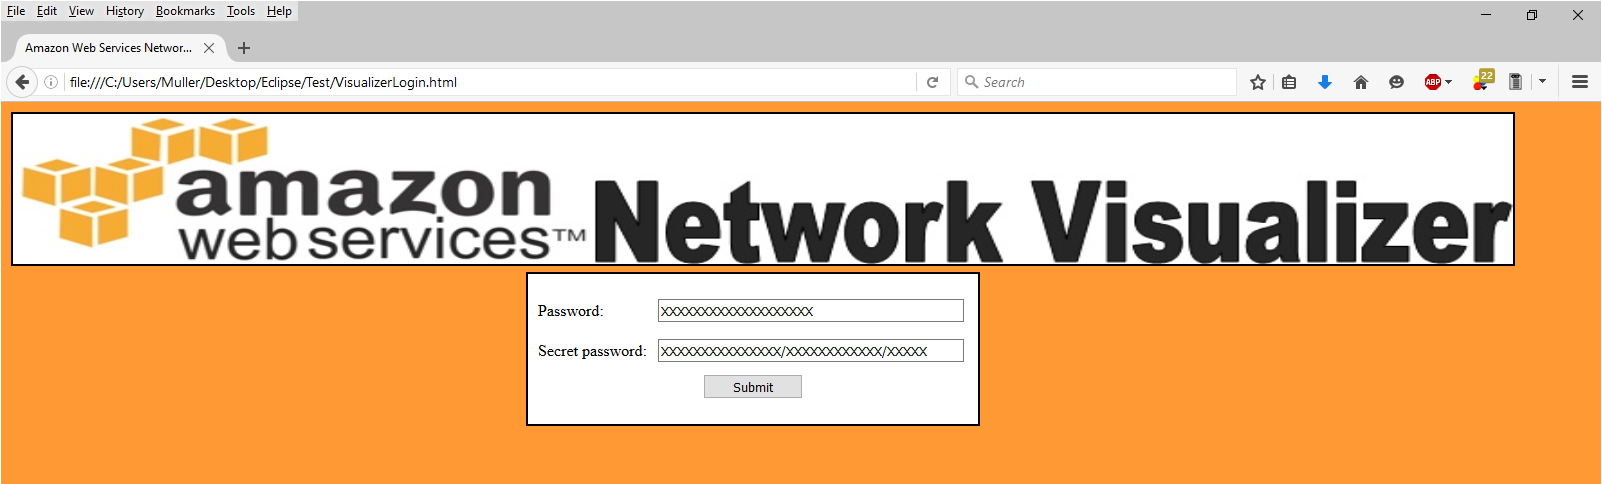
\includegraphics[width=0.9\textwidth]{./images/Login1.png}
    		
    		If the user provides incorrect information, they presented with a message informing them of this ocurrence.
    		
		  	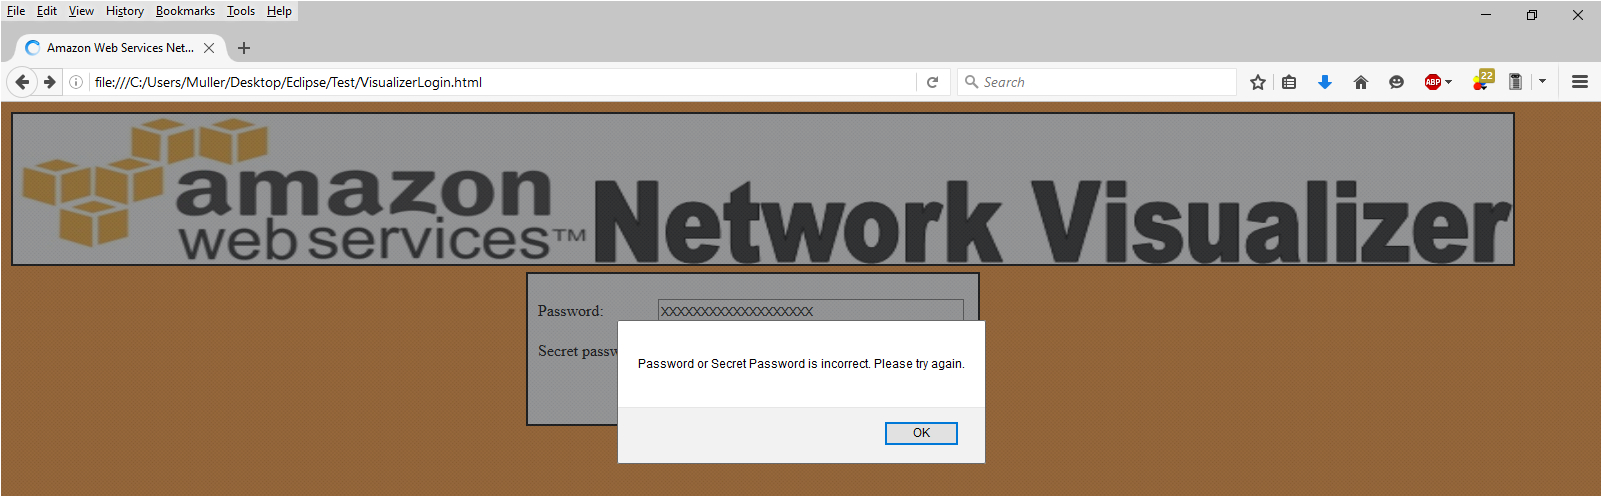
\includegraphics[width=0.9\textwidth]{./images/Login2.png}

	\newpage	
	\subsection{Visualizer}
		This use case pertains to the network visualization. The network is presented in a hierarchial manner, to make traversing the tree easier.
		
		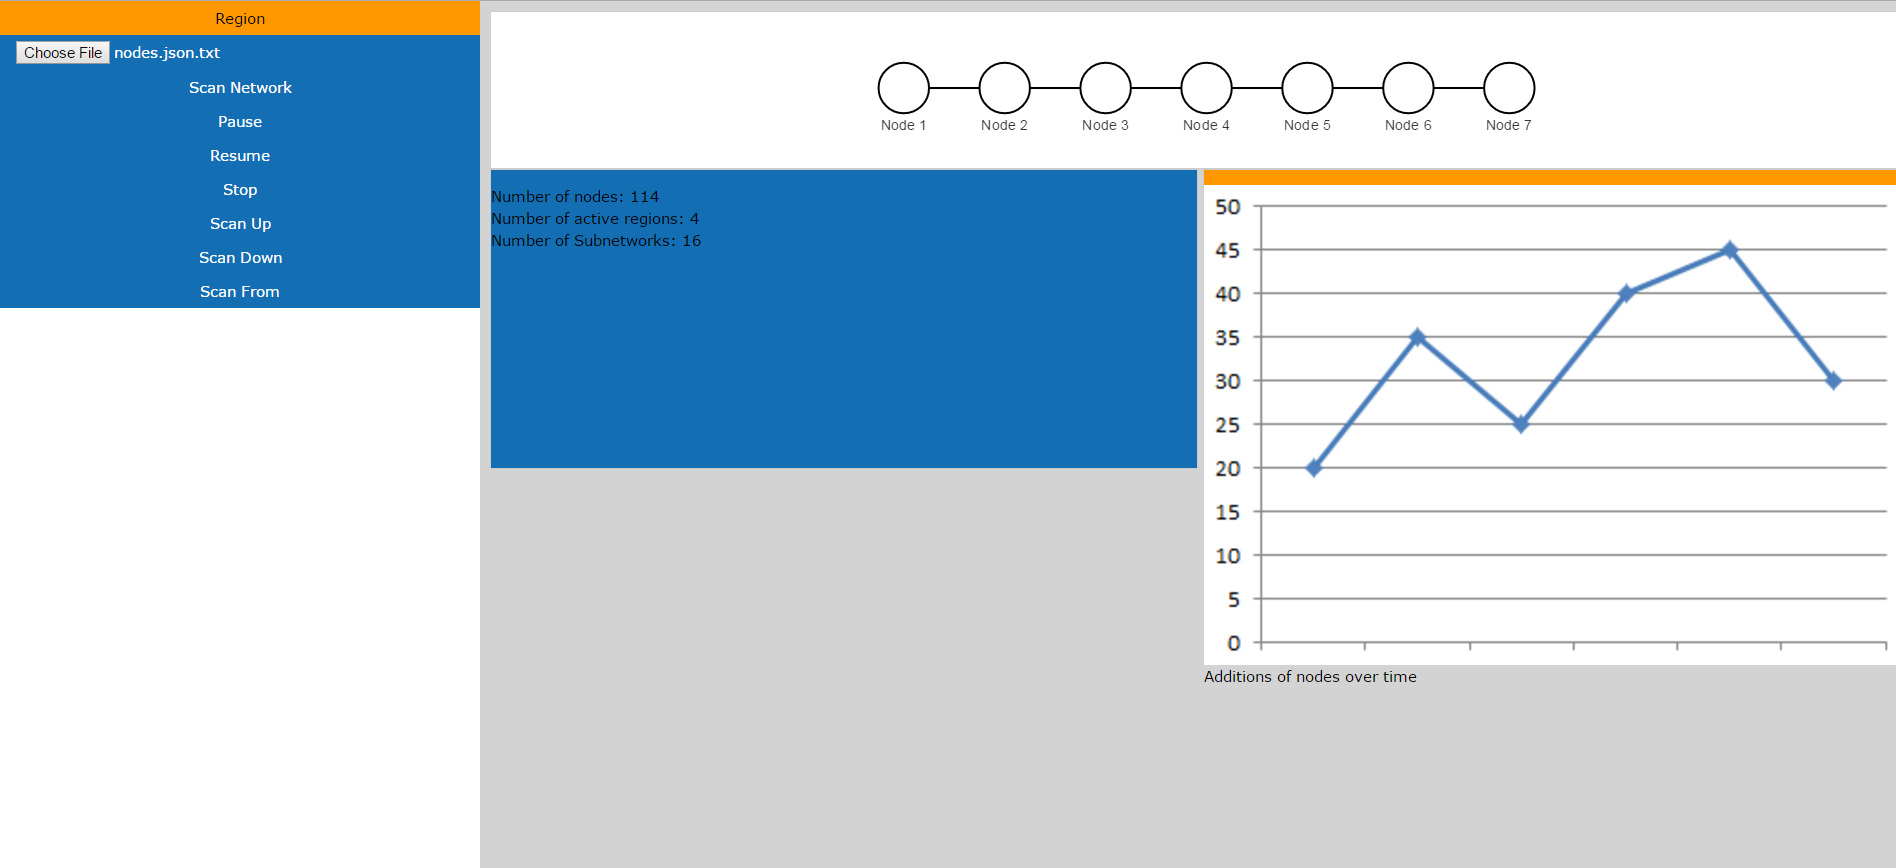
\includegraphics[width=0.9\textwidth]{./images/Visualizer1.png}
	\subsection{Regions}
		The dropdown menu in the left column allows you to select a region to scan. Simply click on a region to scan from there. 
	
		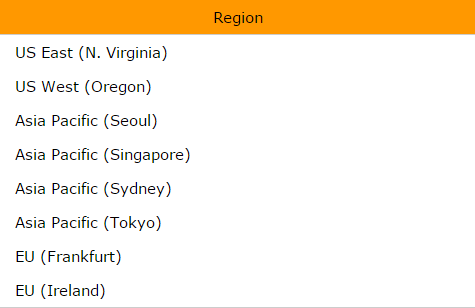
\includegraphics[width=0.9\textwidth]{./images/Visualizer2.png}

	\subsection{Scans}
	There are several scans available to the visualiser, the first being a normal scan for all the regions. 
	
	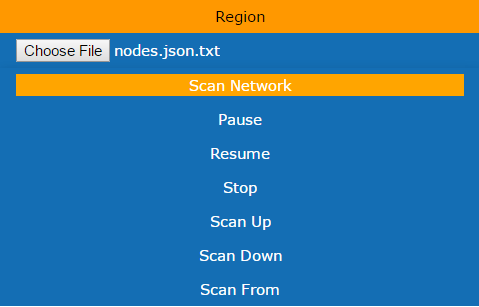
\includegraphics[width=0.9\textwidth]{./images/Visualizer3.png}
	
	You can pause resume and stop a scan via the buttons on the left hand side toolbar. 
	
	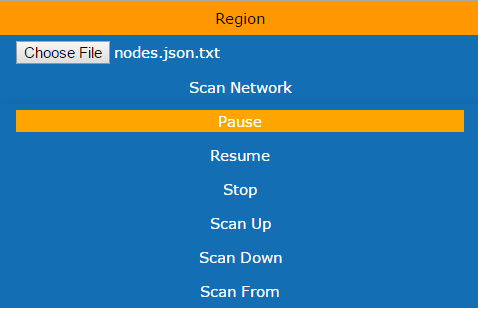
\includegraphics[width=0.9\textwidth]{./images/Visualizer4.png}
	
	You can also scan up and down allowing you to choose which nodes you want prioritized to be scanned. Scan up priorities higher level nodes and scan down priorities lower level nodes. 
	
	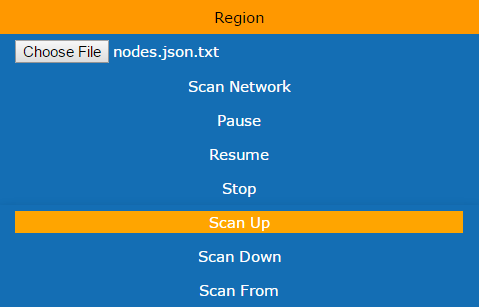
\includegraphics[width=0.9\textwidth]{./images/Visualizer5.png}
	
	Lastly there is a scan from option which lets you select which nodes you would like the scan to start at. 
	
	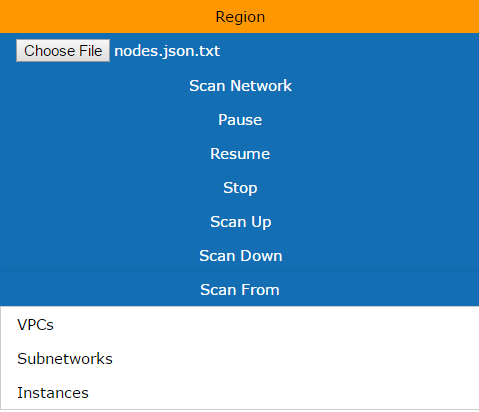
\includegraphics[width=0.9\textwidth]{./images/Visualizer6.png}
	\newpage
	
	\subsection{Zooming}
	Hovering the mouse over the visualizer's window and rolling the mouse wheel will change the zoom of the visualizer. 
	
	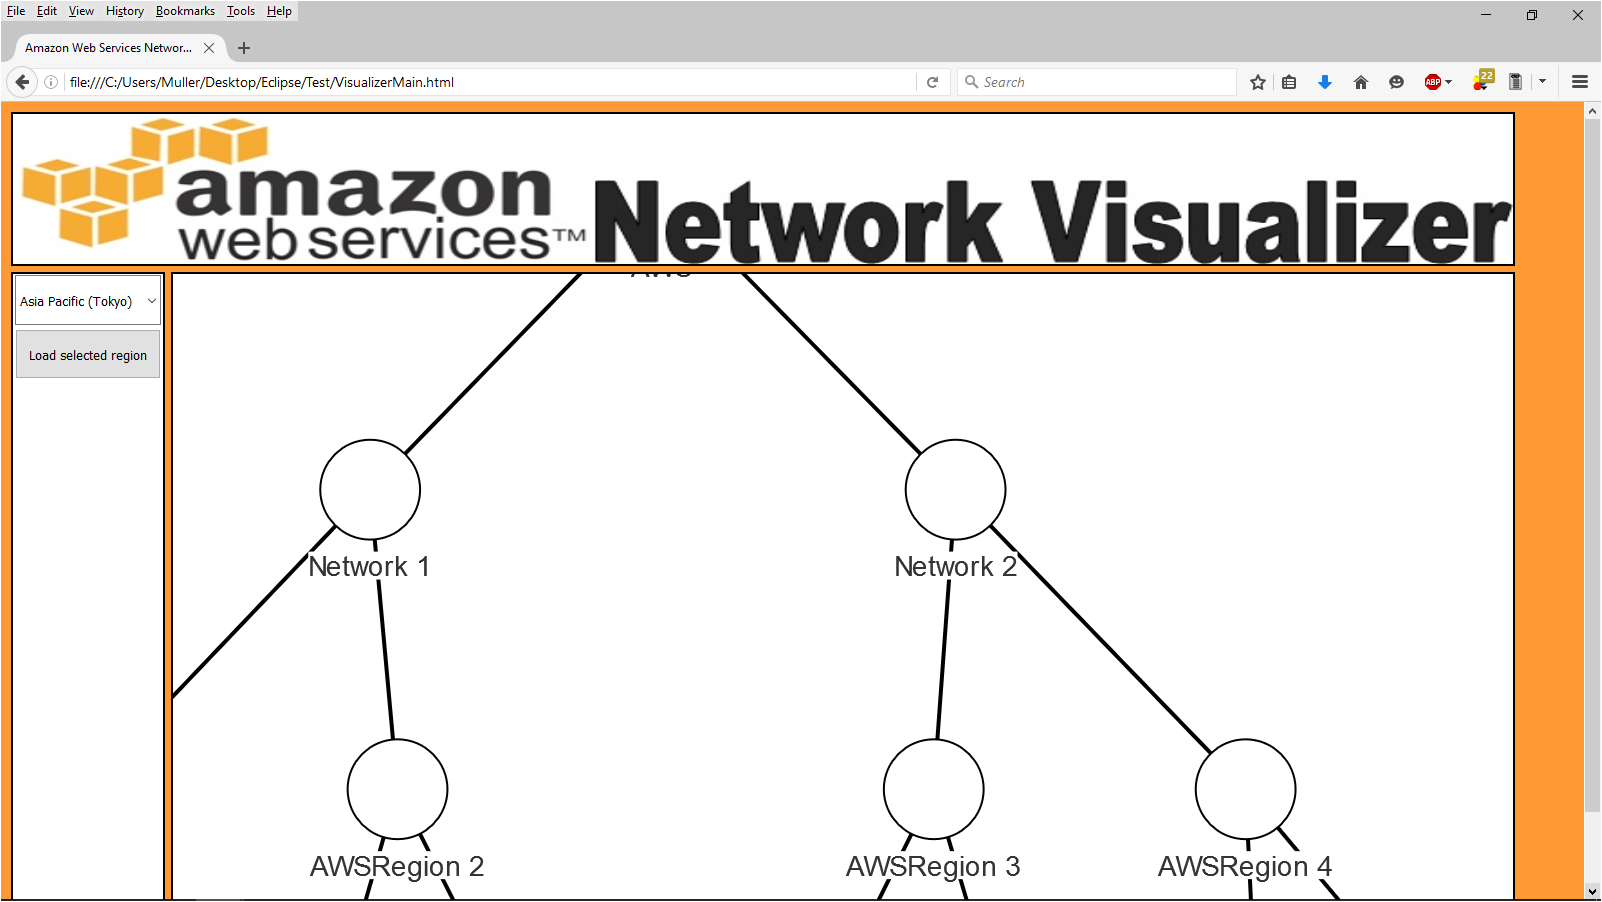
\includegraphics[width=0.9\textwidth]{./images/Visualizer9.png}
	\newpage

	\subsection{Moving}
	Clicking and dragging inside the visualizer's window will move the image.
	
	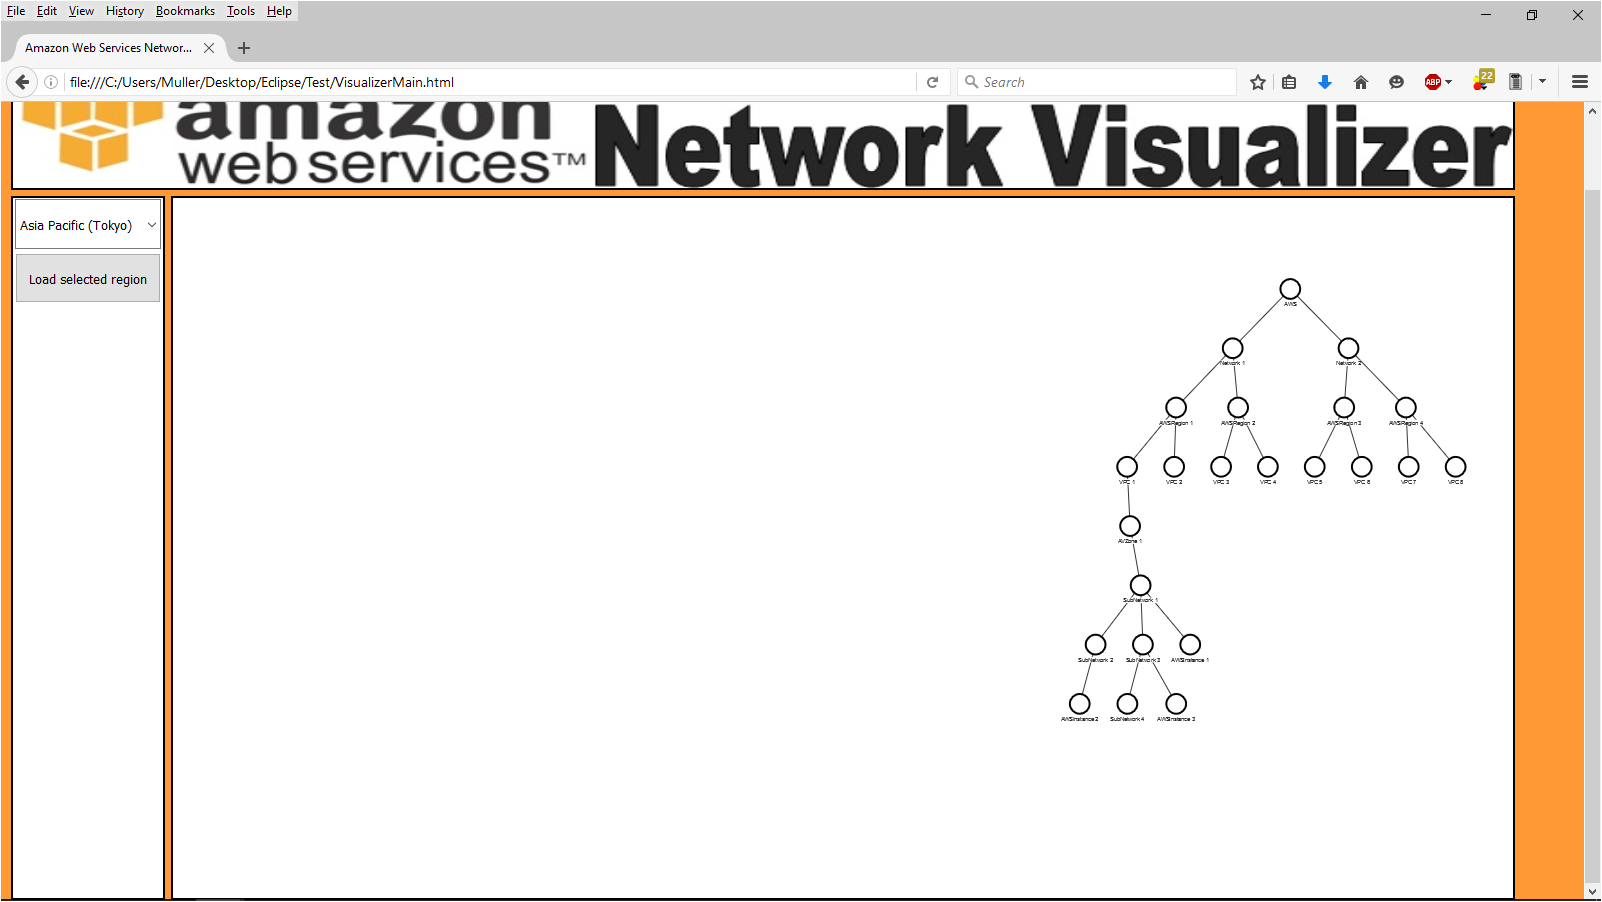
\includegraphics[width=0.9\textwidth]{./images/Visualizer10.png}

	\subsection{Selection}
	Clicking on a node will highlight the selected node and its relationships.
	\newline
		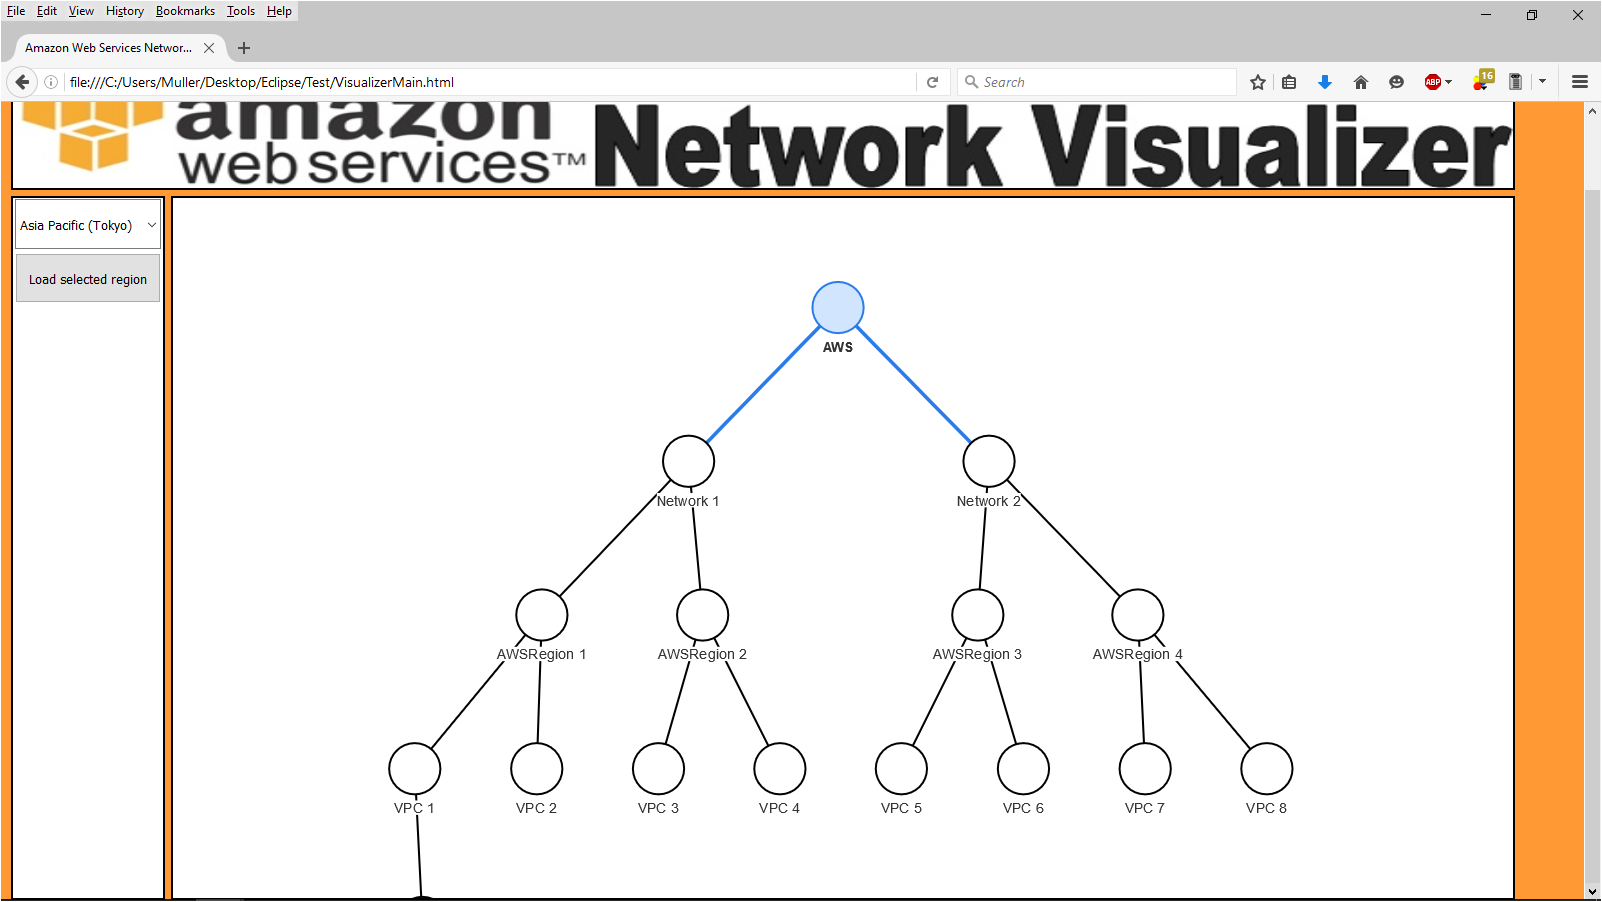
\includegraphics[width=0.9\textwidth]{./images/Visualizer7.png}
		
		\newpage
	\subsection{Information}
	Hovering the mouse over a node will display a small box, specifying its name and the number of VPC's it has.
	
	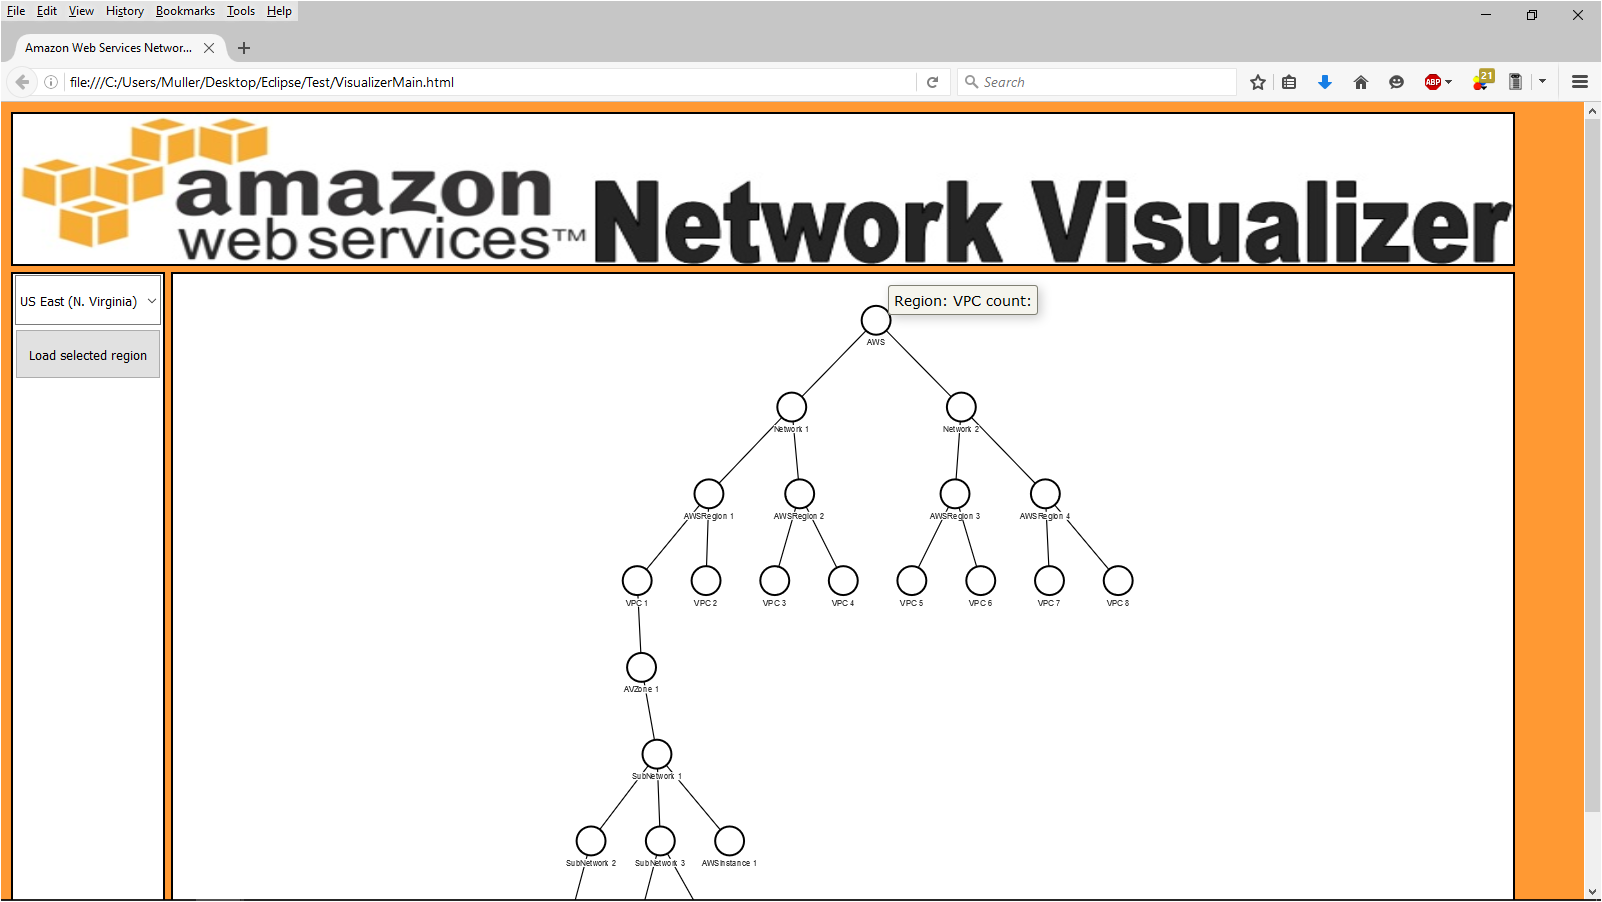
\includegraphics[width=0.9\textwidth]{./images/Visualizer8.png}
	\newline
	

\end{document}
